\documentclass[12pt]{article}
%%%%%%%%%%%%%%%%%
% Imported Packages
%%%%%%%%%%%%%%%%%
\usepackage{setspace}
\usepackage{url}
\usepackage{multicol}
\usepackage{etoolbox}
\usepackage{relsize}
\patchcmd{\thebibliography}
  {\list}
  {\begin{multicols}{2}\smaller\list}
  {}
  {}
\appto{\endthebibliography}{\end{multicols}}

\usepackage{titlesec}
\usepackage{flushend}
\expandafter\def\expandafter\UrlBreaks\expandafter{\UrlBreaks%  save the current one
  \do\\\do-}

\usepackage{soul}

\usepackage{graphicx}
\graphicspath{ {images/} }

\usepackage{capt-of}

%%% PAGE DIMENSIONS
\usepackage[top=4.5cm, bottom=4.5cm, left=2cm, right=2cm]{geometry}
\usepackage{geometry} % to change the page dimensions
\geometry{letterpaper}

\begin{document}


%%%%%%%%%%%%%%%
% Title
%%%%%%%%%%%%%%%
\title{\vfill LiteCrypto} %\vfill gives us the black space at the top of the page
\author{
Team AES - Andrew Wang, Sam (Jiewen) Wu, and Elton Yang \vspace{10pt} \\
CPE 458: Current Topics in Computer Systems (Cryptographic Engineering)  \vspace{10pt} \\
Dr. Zachary Peterson \vspace{10pt} \\
}
\date{December 12, 2014} %Or use \today for today's Date

\maketitle

\vfill  %in combination with \newpage this forces the abstract to the bottom of the page
\begin{abstract}
\end{abstract}
\thispagestyle{empty} %remove page number from title page, but still keep it as pg #1
\newpage
\thispagestyle{empty}
\tableofcontents
\thispagestyle{empty}
\mbox{}
\newpage

%%%%%%%%%%%%%%%%%%%%
%%% Known Facts  %%%
%%%%%%%%%%%%%%%%%%%%
\begin{multicols}{2}
\section{Introduction}
\subsection{CubeSat}
CubeSat is a international collaborative project of over 40 educational systems and private firms. A CubeSat is a satellite that is 10 cm3 and with a mass of 1.33 kg. 
\subsection{PolySat}
PolySat is Cal Poly’s branch of CubeSat, and was established since 1999. Dr. Bellardo is the current advisor for PolySat. They have eight launched missions and three are currently in development. 
\section{Motivation and Background}
Our group decided on creating a CubeSat Crypto Library for our Crypto Engineering Final Project. 
\subsection{Background}
Dr. Bellardo has discussed with our team that the future of CubeSat is to allow them to move in space. However, their current communications from home base to the satellite is encrypted and unauthorized.  Therefore, an adversary who wishes to harm the CubeSat, or harm another object using the CubeSat, may sniff a command packet to the satellite and control it. Dr. Bellardo has given us a set of requirements that the library should have.
\subsection{Requirements}
\subsubsection{Binary Size}
Due to the small size of the CubeSat and the large amount of things it does, there is not a lot of storage space for the library. Therefore, the binary size needed to be around 50 kilobytes. Because the library would be part of its main functions, it will also need to be small for a quick boot time for the operating system. 
\subsubsection{Data Transfer}
Our library can not use transfer large amount of data between home base and the satellite. AX.25 speed limits on data are rarely higher than 9,600 bits/s and are usually 1,200 bits/s. The satellite also does not return an acknowledgement packet after successful retrieving a packet. Therefore, we are restricted on which scheme to use for our crypto library. Another issue is the connection time with the CubeSat is at most 15 minutes an hour due to the satellite orbiting the Earth. Therefore, we cannot use schemes that require a constant connection with the satellite. 
\subsubsection{Encryption and Authentication}
Our library should allow any user to have the option to encrypt or authenticate their packets. It should have 3 functions: No security, one way authentication, and authenticated encryption. Using the diagram below is how Dr. Bellardo described how we should encrypt and authenticate. \\
\begingroup
    \centering
    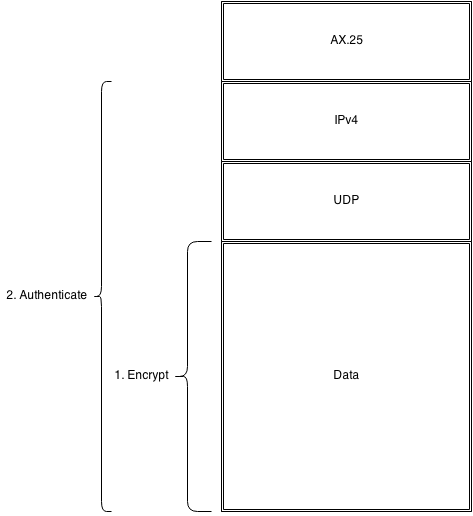
\includegraphics[width=7cm]{researchDiagram.png}
\endgroup
We were told to only encrypt the data portion of the packet, and only authenticate the IPv4 and UDP headers along with the data.
\section{Related Work/Research}
We began our research by looking for current satellite encryption. We found a paper on AES (Advanced Encryption Standard) with LDPC (Low Density Parity Check Code) in order to design a secure and reliable error correction method. \cite{SEEC} We also found that stream ciphers lead to serious problems if used incorrectly for satellite applications. \cite{stream_problems} We discovered someone else's work to authenticate IP protocol. \cite{IP_Protocol} In order to meet the low overhead requirement we found a low cost one-way HMAC proposal for a RFID system. \cite{HMAC_RFID} With all of this information, we needed a light weight software library for encryption to use. 
\subsection{CyaSSL (wolfSSL)}
CyaSSL is a lightweight SSL/TLS library. It advertised a special build called LeanPSK, which was an implementation of CyaSSL that could be built in as little as 20 kilobytes. LeanPSK is also 20 times smaller than OpenSSL, and uses 1 to 36 kilobytes of memory. This configuration required pre-shared keys. However, after creating the binary ourselves and using their library, we found it to be complicated to build and the binary ended up to be 57 kilobytes. That was above our binary size requirement so we looked for a different library to use. 
\subsection{NaCl}
The NaCl crypto library has all of the core operations needed to build our crypto library. NaCl advertises state of the art security, improves usability, and improved speed. However the full NaCl library is too large for us to use, so we found a smaller version of the NaCl library to use.
\subsubsection{TweetNaCl}
TweetNaCl supports 25 of the C NaCl functions used by applications and fits into a 100 tweets. It is self contained library so it was easy to build. However, it did not have HMAC build into TweetNaCl so we ported it from the original NaCl library.
\section{Our Work}
\section{Evaluation and Analysis}
\section{Conclusion}
\end{multicols}
\end{document}
